\subsection{Klassediagram}
For at illustrere modellaget i vores MVC-mønster, har vi produceret et klassediagram (se \myref{diagram:klassediagram} nedenfor) i UML, der simplificerer strukturen. 
Dette diagram er en implementation af vores struktur fra problemområdeanalysen på \myref{figur:PDklasse}.

\begin{figure}[h]
\centering
 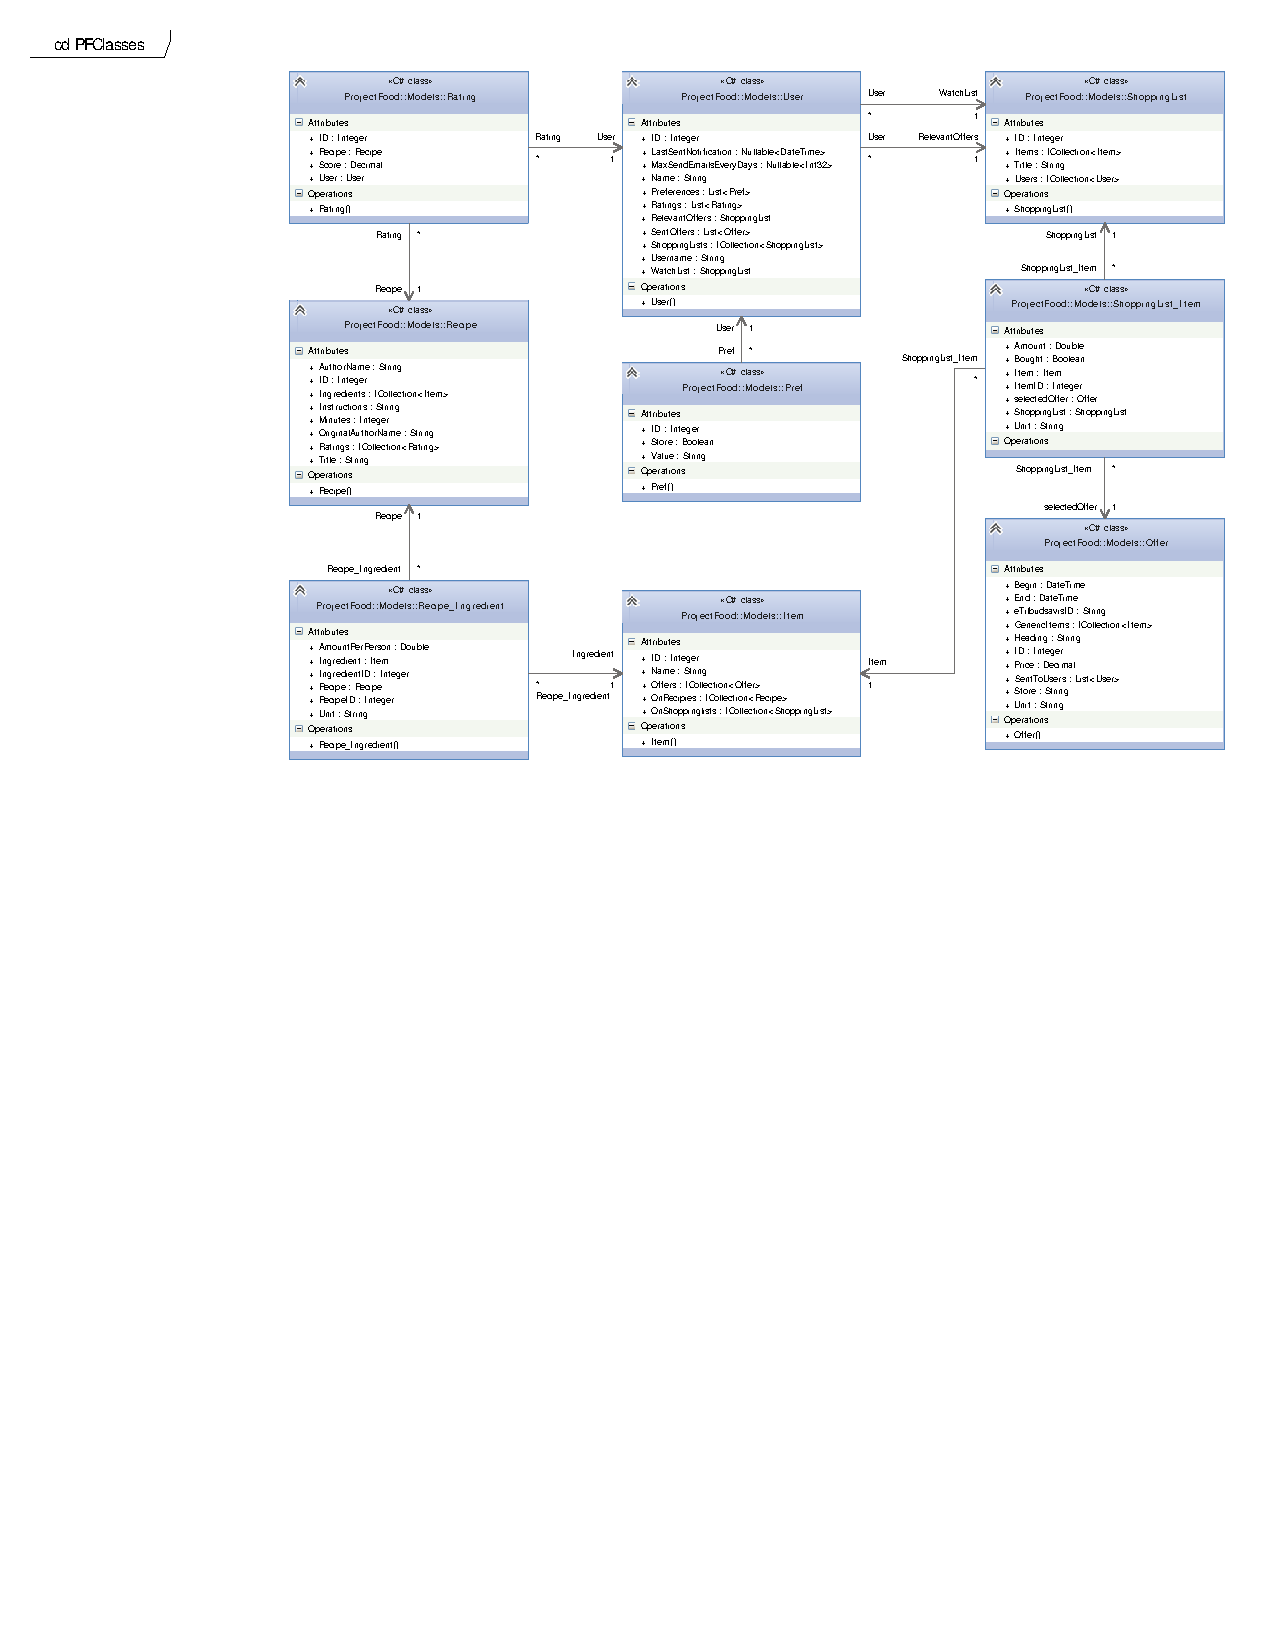
\includegraphics[trim=4.85cm 15cm 0.85cm 1cm, clip, width=1\textwidth]{/Diagrams/PFClasses.pdf}
\caption{UML klassediagram for modellaget i MVC-mønsteret}\label{diagram:klassediagram}
\end{figure}

Der er mange relationer mellem klasserne, da de forskellige klasser indeholder lister af hinanden.
En ShoppingList har en liste over Items, og disse Items har en liste over Offers, for at binde Offers til det pågældende Item.
Recipe har en liste over Items, som bruges som ingredienser.
På denne måde kan de tilføjes til ShoppingList gennem RecipesController, uden at skulle lave nye objekter, som ShoppingList kan læse.
User har en liste over ShoppingLists, samt en liste over Prefs, eller præferencer som angiver hvilke tilbud der skal filtreres væk, for at gøre hjemmesiden mere personlig og fokuseret på brugeren som er logget ind.
Der er relationstabeller mellem many-to-many forholdene, som yderligere gør det muligt at gemme værdier ved hvert forhold, eksempelvis mængder (``Amount'') på en ShoppingList.
Dette gøres igennem relationsklasserne, Recipe\textunderscore Ingredient, og ShoppingList\textunderscore item.

I de følgende afsnit, vil der gives en gennemgang af udvalgte dele af komponenterne fra \myref{subsec:komp}.
